\subsection{Performance of the Filter}
The position Kalman filter is tested in a similar way as the attitude one. The simulations have been performed by applying some inputs to the simulation model of the system. The signals coming out of the model are then extracted and some noise is added to them. The noisy signals are used as the input to the position Kalman filter in order to evaluate its performance. The amount of noise added is the same as that present in the real sensors, the variance values can be seen in \autoref{app:IMUVariances}.

In \autoref{fig:sim_xn}, the results for $x_\mathrm{n}$ can be seen. The position of the vessel is precisely estimated with the Kalman filter that removes most of the noise comming from the sensed data.

\begin{figure}[H]
    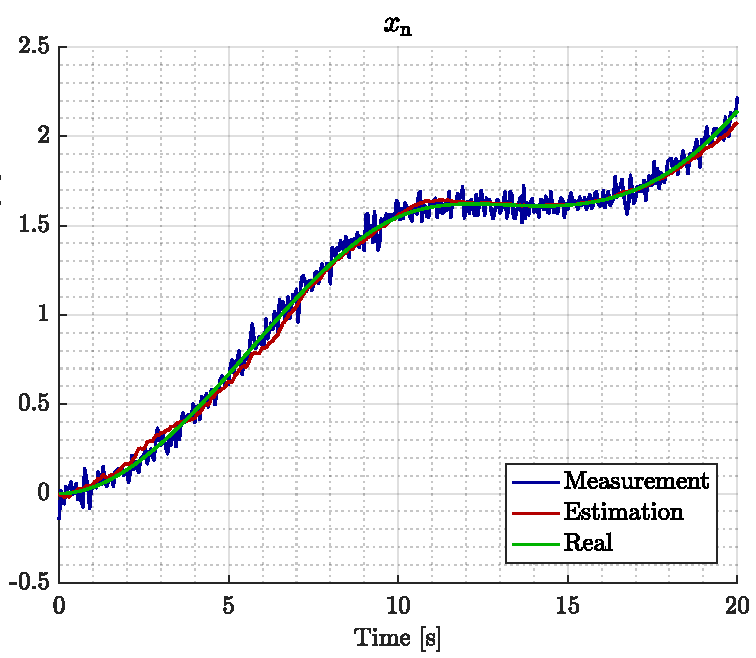
\includegraphics[width=0.5\textwidth]{figures/sim_xn}
    \caption{Measurement, real value and estimation of $x_\mathrm{n}$.}
    \label{fig:sim_xn}
\end{figure}

The vessel velocity $\dot{x}_\mathrm{b}$ is not directly measured in the system. In \autoref{fig:sim_xbdot} it is shown how the Kalman filter correctly estimates it and how it follows the real value obtained from the simulation.

Finally, the estimation of $\ddot{x}_\mathrm{b}$ is shown in \autoref{fig:sim_xbddot}. It can be seen that the estimated acceleration follows the real value and the noise present is reduced with respect to that present in the measurement.

\begin{figure}[H]
    \captionbox 
    {   
        Real value and estimation of $\dot{x}_\mathrm{b}$.
        \label{fig:sim_xbdot}
    }                                                                 
    {                                                                  
        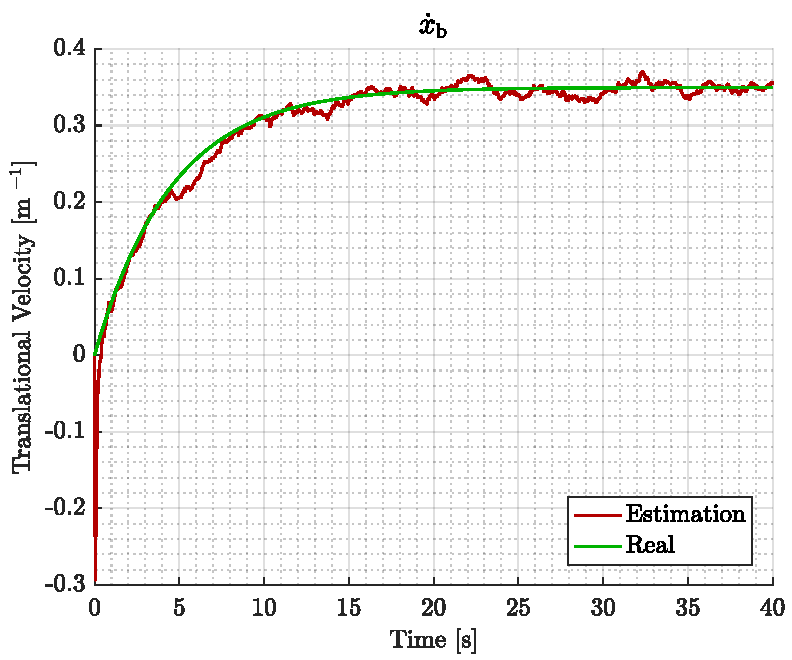
\includegraphics[width=.45\textwidth]{figures/sim_xbdot}         
    }                                                                    
    \hspace{5pt}                                                          
    \captionbox  
    {      
        Real value and estimation of $\ddot{x}_\mathrm{b}$.
        \label{fig:sim_xbddot}
    }                                                                          
    {
        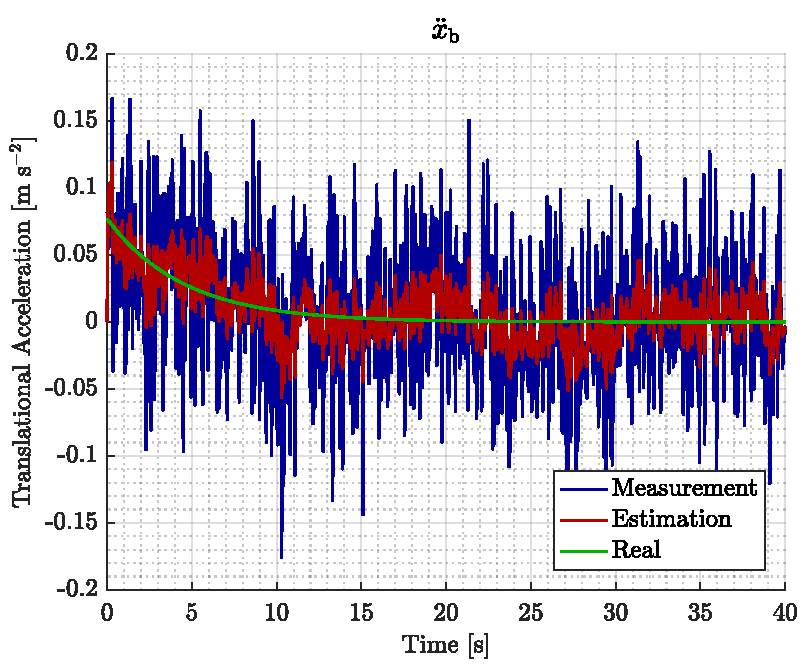
\includegraphics[width=.45\textwidth]{figures/sim_xbddot}
    }
\end{figure}

The evaluation of both Kalman filters performance in simulations has been carried successfully, as well as the inner and outer controller designs. In Part II a brief description of the implementation in the system is presented, as long as the results and conclusion of the project.